% Kites Vector Extension (RVV 1.0) - Validation Report
% Build: tectonic validation_report.tex   (or: make)
\documentclass[11pt]{article}
\usepackage{kitesdoc}
\usepackage{graphicx}
\usepackage[capitalise,noabbrev]{cleveref}
\renewcommand{\kdocshorttitle}{Kites Vector Extension --- Validation}
\hypersetup{pdftitle={Kites Vector Extension (RVV 1.0): Validation Report}}
\newcommand{\pass}{\textcolor{kstretch}{\textsf{\textbf{pass}}}}
\newcommand{\partly}{\textcolor{kshould}{\textsf{\textbf{partial}}}}

\begin{document}

% =====================================================================  TITLE
\begin{titlepage}
\thispagestyle{empty}
\vspace*{1.2cm}
{\sffamily\small\color{kgrey} CS2323 Computer Architecture \quad$\cdot$\quad IIT Hyderabad}\par
\vspace{0.6cm}
{\sffamily\bfseries\fontsize{26}{31}\selectfont\color{kblue} Vector Extension Support\\[2pt] for the Kites RISC-V Simulator\par}
\vspace{0.5cm}
{\sffamily\Large\color{kteal} Validation Report\par}
\vspace{0.2cm}
{\large RISC-V ``V'' extension 1.0, the Zve* subsets, and the Zvfh, Zvbb/Zvkb and Zvbc extensions\par}
\vspace{1.4cm}

\begin{tabularx}{\textwidth}{@{}L{3.6cm}Y@{}}
\toprule
\textsf{\textbf{Document}}   & Validation report \\
\textsf{\textbf{Version}}    & 1.0 \\
\textsf{\textbf{Author}}     & Raam M \\
\textsf{\textbf{Repository}} & \url{https://github.com/Raam-M/Kites}, branch \texttt{vector-extension} \\
\textsf{\textbf{Environment}} & macOS 26 (arm64), Apple Clang 15, Qt 6, Spike 1.1.1-dev, LLVM \texttt{llvm-mc} \\
\textsf{\textbf{Companions}} & Scope document (requirements, quality gates); design document \\
\bottomrule
\end{tabularx}

\vspace{1.0cm}
\begin{keybox}[title=Purpose of this document]
This report records how the vector extension was validated against the plan in the scope
document, and the results: unit and integration tests, differential testing against Spike,
coverage, performance, the GUI checks, the defects found, a requirement-to-test traceability
matrix and the status of each quality gate.
\end{keybox}
\vfill
\end{titlepage}

\tableofcontents
\clearpage

% =====================================================================  1
\section{Summary}\label{sec:summary}

\begin{table}[H]
\centering\small
\caption{Results at a glance.}\label{tab:glance}
\begin{tabularx}{\textwidth}{@{}L{5.2cm}Y@{}}
\toprule
Measure & Result \\
\midrule
Automated tests (CTest) & 261 of 261 pass: 103 new vector and pipeline tests, 158 existing tests \\
Instructions covered & 647 table entries (627 V, 20 Zvbb/Zvkb/Zvbc), each with an \texttt{llvm-mc} golden encoding; semantic tests for every instruction family \\
Differential testing vs Spike & 2\,405 programs, 0 mismatches: 55 example runs and 2\,350 random programs over 20 configurations (\cref{tab:spike}) \\
Line / branch / function coverage & 95.2\,\% / 88.5\,\% / 98.7\,\% of the new vector code (targets: 90\,\% lines, 75\,\% branches) \\
Scalar performance (NF-01) & per instruction faster than before (CPU time $-4.4$\,\% and $-6.4$\,\% on the longer programs); about 3\,ms more start-up (\cref{sec:perf}) \\
Quality gates & QG1--QG4, QG6 and QG7 met; QG5 met on macOS, Linux not run (\cref{sec:gates}) \\
\bottomrule
\end{tabularx}
\end{table}

All compulsory requirements (tiers A1 and A2) and all stretch goals (B1--B10) are implemented
and verified. Validation found nine defects in the existing Kites code, six of which are fixed
(\cref{sec:defects}). The differences from Spike that the specification allows are handled
explicitly (\cref{sec:spike-diff}).

% =====================================================================  2
\section{Validation levels}\label{sec:levels}

\small
\begin{longtable}{@{}L{0.9cm}L{3.0cm}L{9.2cm}L{1.6cm}@{}}
\caption{Validation levels of the scope document and what was done.}\label{tab:levels}\\
\toprule
Level & Focus & Done & Status \\
\midrule
\endfirsthead
\caption[]{Validation levels (continued).}\\
\toprule
Level & Focus & Done & Status \\
\midrule
\endhead
L1 & Units & vtype, VLMAX, legality helpers, rounding, saturation, \texttt{rec7}/\texttt{rsqrt7}, high multiplies, half rounding, configuration parsing, element formatting & \pass \\
L2 & Assembler & 1\,293 \texttt{llvm-mc} golden encodings; decode and disassembly round trip; error messages; labels named like vtype fields; pseudo-instructions & \pass \\
L3 & Semantics & every family against an independent reference model over all 22 SEW/LMUL pairs, \texttt{vl} values, masks, policies, \texttt{vstart}; FP edge values; half precision against hardware \texttt{\_Float16} & \pass \\
L4 & Legality & every rule raises an error and leaves all state bit-identical & \pass \\
L5 & Programs & 11 example programs checked against expected values and scalar versions, at every VLEN and on the pipelines & \pass \\
L6 & Differential & Spike, 2\,405 programs over 20 configurations (\cref{sec:spike}) & \pass \\
L7 & System & undo/redo round trips (single-cycle and pipeline), reset, retirement counting, statistics undo & \pass \\
L8 & Regression & full existing suite; macOS & \partly \\
L9 & Coverage & clang source-based coverage (\cref{sec:coverage}) & \pass \\
L10 & GUI & offscreen renders of the new views, checklist (\cref{sec:gui}) & \pass \\
\bottomrule
\end{longtable}
\normalsize

% =====================================================================  3
\section{Automated tests}\label{sec:tests}

\Cref{tab:suites} lists the new test suites. Test names begin with the requirement they verify
(for example \texttt{VM02\_\ldots} for VM-02). Expected values come from an independent
reference model (\file{test/vector/vector_reference.h}), from \texttt{llvm-mc}, from the hardware's
\texttt{\_Float16} conversions, from hand calculation, or from the single-cycle processor when a
pipeline is checked.

\small
\begin{longtable}{@{}L{3.4cm}L{1.0cm}L{6.9cm}L{2.7cm}@{}}
\caption{New test suites (\texttt{test/vector/}, \texttt{test/rv5s\_regression\_test.cpp}).}\label{tab:suites}\\
\toprule
Suite & Tests & Covers & Oracle \\
\midrule
\endfirsthead
\caption[]{New test suites (continued).}\\
\toprule
Suite & Tests & Covers & Oracle \\
\midrule
\endhead
VecAsm & 12 & golden encodings, decode, round trip, inventory, syntax errors, vtype forms, labels, CSR and vector pseudos & \texttt{llvm-mc} \\
VecConfig & 7 & reset state, \insn{vset*}, \texttt{x0} cases, \texttt{vill}, vector CSRs, \texttt{vstart} & spec rules \\
VecInteger & 9 & single-width, division, multiply-add, widening, narrowing, extension, carry, compare, merge & reference model \\
VecPermute & 7 & reductions, mask operations, \insn{viota}/\insn{vid}, scalar moves, slides, gather, compress, whole-register moves & reference model \\
VecMemory & 5 & unit-stride, strided, indexed, mask, whole-register, fault-only-first, cache traffic & reference model \\
VecFloat & 8 & FP arithmetic, FMA, compares, special values and flags, conversions, estimates, reductions, legality & host IEEE, spec tables \\
VecHalf & 5 & Zvfh in all rounding modes, FMA forms, integer conversions, flags; element formatting & hardware \texttt{\_Float16} \\
VecExtensions & 11 & Zvbb, Zvbc, disabled extensions, Zve* profiles, option parsing, Zvfh values, VLEN, agnostic fill & reference model \\
VecLegality & 4 & group, overlap, \texttt{vill}, \texttt{vstart} rules; state unchanged & spec rules \\
VecSystem & 2 & undo/redo round trip, retirement & recorded state \\
VecExamples & 11 & the example programs & expected values, scalar code \\
VecPipeline & 10 & examples and dependent chains on the pipelines, stall cycles, NOP rule, memory order, flushing, errors in WB, undo/redo, FP ordering & single-cycle model \\
VecProfiler & 5 & statistics, classification, hand-computed schedules, structural hazards, undo & hand calculation \\
VectorCustomPseudo & 3 & vector expansions: accepted, rejected, expanded and run & expected values \\
Rv5sRegression & 4 & AUIPC/LUI, \insn{la}, FP integer-source forwarding, draining & expected values \\
\bottomrule
\end{longtable}
\normalsize

\paragraph{Mutation checks.} To confirm that the tests detect defects, deliberate faults were
inserted and the tests were run, then removed. For example, removing the stall for scalar
instructions that depend on a vector result made four pipeline tests fail; in one of them a
strip-mined loop no longer terminated, which the test reports through its step limit.

% =====================================================================  4
\section{Differential testing against Spike}\label{sec:spike}

\subsection{Harness}
\file{tools/vector/spike_diff.py} runs the same program on Kites and on Spike~\cite{spike}. A
shared epilogue stores the final architectural state into a dump area next to the program data:
\texttt{x1}--\texttt{x31}, \texttt{f0}--\texttt{f31}, \texttt{v0}--\texttt{v31}, \texttt{vl},
\texttt{vtype}, \texttt{vxsat}, \texttt{vxrm}, \texttt{fflags} and \texttt{frm}. Kites runs the
program through \texttt{kites-cli} and dumps memory; Spike runs an ELF built with
\texttt{llvm-mc} and \texttt{ld.lld} and writes the same region with \texttt{+signature}. The data
memory, vector registers, vector CSRs, \texttt{fflags} and the scalar registers the program uses
are compared byte for byte. The harness selects the Kites processor model, VLEN, profile and
extensions, and passes the matching ISA string to Spike (for example
\texttt{rv64gc\_zve64f\_zfhmin\_zvfh\_zvl128b}).

Random programs are generated from a seed. A prologue loads random data with edge values (zeros,
all ones, sign boundaries, infinities, NaNs, subnormals) into all vector and FP registers and
sets the scalar operands; the body draws from every instruction family: integer, multiply-add,
compares, widening, narrowing, extension, carry, merges, reductions, mask operations,
permutations, fixed-point rounding modes, floating point (including conversions at every legal
width and rounding modes), loads and stores of every kind, \insn{vset*} with random AVL, SEW and
LMUL, and the Zvbb/Zvkb/Zvbc instructions. Only instructions legal for the target configuration
are generated. A failing program can be bisected to the first line where the states diverge.

\subsection{Results}

\small
\begin{longtable}{@{}L{2.0cm}L{1.8cm}L{1.2cm}L{4.4cm}L{1.6cm}L{2.0cm}@{}}
\caption{Final campaign: every program matches Spike.}\label{tab:spike}\\
\toprule
Run & Processor & VLEN & Profile, extensions & Programs & Matching \\
\midrule
\endfirsthead
\caption[]{Final campaign (continued).}\\
\toprule
Run & Processor & VLEN & Profile, extensions & Programs & Matching \\
\midrule
\endhead
examples & single-cycle & 128 & V & 11 & 11 \\
examples & single-cycle & 512 & V & 11 & 11 \\
examples & H\_NF & 128 & V & 11 & 11 \\
examples & H\_F & 128 & V & 11 & 11 \\
examples & H\_F & 1024 & V & 11 & 11 \\
random & single-cycle & 128 & V & 500 & 500 \\
random & single-cycle & 256 & V & 150 & 150 \\
random & single-cycle & 512 & V & 150 & 150 \\
random & single-cycle & 1024 & V & 150 & 150 \\
random & single-cycle & 128 & V, Zvfh, Zvbb, Zvbc & 300 & 300 \\
random & single-cycle & 256 & V, Zvfh, Zvbb, Zvbc & 100 & 100 \\
random & single-cycle & 128 & V, Zvkb & 50 & 50 \\
random & single-cycle & 128 & Zve64d & 100 & 100 \\
random & single-cycle & 128 & Zve64f, Zvfh & 100 & 100 \\
random & single-cycle & 128 & Zve64x, Zvbb, Zvbc & 100 & 100 \\
random & single-cycle & 128 & Zve32f, Zvfh & 100 & 100 \\
random & single-cycle & 128 & Zve32x, Zvkb & 100 & 100 \\
random & H\_NF & 128 & V & 150 & 150 \\
random & H\_F & 128 & V & 200 & 200 \\
random & H\_F & 256 & V, Zvfh, Zvbb, Zvbc & 100 & 100 \\
\midrule
total & & & & 2\,405 & 2\,405 \\
\bottomrule
\end{longtable}
\normalsize

Each random program has 40 instructions after the prologue (about 60 to 120 executed
instructions including the prologue, the epilogue and expansions). The models without hazard
detection (NH\_NF, NH\_F) are not in the random campaign, because the random programs do not
contain the NOPs those models need; they are covered by \texttt{PL02} and the existing pipeline
tests.

\subsection{Allowed differences}\label{sec:spike-diff}

The specification lets implementations differ in some places. The harness avoids these cases,
or Kites makes the same choice as Spike:

\begin{description}[style=nextline,leftmargin=0.6cm,font=\sffamily\bfseries\color{kblue}]
\item[Agnostic elements] Kites leaves them undisturbed by default, as Spike does; the all-ones
  fill is verified by unit tests (VC-04).
\item[Misaligned element accesses] Spike traps on a misaligned strided element access, Kites
  allows it (D8). Random strides are multiples of the element size.
\item[NaN-boxing] Spike treats a single or half value that is not NaN-boxed as the canonical NaN;
  Kites reads the low SEW bits (F18). The harness loads NaN-boxed scalars, which both read the
  same way. FP registers are not compared.
\item[Unordered sums] Both add in element order. With no active element and a NaN scalar,
  Spike returns the canonical NaN; Kites originally returned the scalar unchanged. Both are
  allowed; Kites now makes the same choice (found by the campaign at VLEN=256, seed 6062).
\end{description}

% =====================================================================  5
\section{Coverage}\label{sec:coverage}

The test suite was built with clang source-based coverage (\texttt{-fprofile-instr-generate
-fcoverage-mapping}) and the profiles were merged with \texttt{llvm-profdata}. The project's
existing \texttt{coverage} target links GCC's \texttt{libgcov}, which Apple Clang does not
provide, so it was not used. Coverage counts only the unit and integration tests; the Spike
campaigns run through \texttt{kites-cli} and add to the confidence but not to these numbers.

\begin{table}[H]
\centering\small
\caption{Coverage of the new vector code.}\label{tab:coverage}
\begin{tabularx}{\textwidth}{@{}YL{2.1cm}L{2.3cm}L{2.0cm}@{}}
\toprule
File & Lines & Branches & Functions \\
\midrule
\file{vector_exec_integer.cpp} & 99.7\,\% & 98.3\,\% & 100\,\% \\
\file{vector_unit.cpp} & 97.0\,\% & 92.1\,\% & 100\,\% \\
\file{vector_exec_memory.cpp} & 94.7\,\% & 90.6\,\% & 100\,\% \\
\file{vector_exec_float.cpp} & 92.0\,\% & 81.0\,\% & 98.4\,\% \\
\file{vector_isa.cpp} & 92.7\,\% & 89.2\,\% & 92.9\,\% \\
\file{vector_config.cpp} & 94.9\,\% & 92.2\,\% & 100\,\% \\
\file{vector_profiler.cpp} & 98.5\,\% & 91.5\,\% & 93.3\,\% \\
\file{vector_format.cpp} & 98.9\,\% & 90.0\,\% & 100\,\% \\
\file{vtype.cpp} & 95.0\,\% & 89.3\,\% & 100\,\% \\
\file{v_formats.cpp} (assembler) & 90.3\,\% & 78.6\,\% & 100\,\% \\
headers & 100\,\% & 100\,\% & 100\,\% \\
\midrule
\textbf{total} & \textbf{95.2\,\%} & \textbf{88.5\,\%} & \textbf{98.7\,\%} \\
\bottomrule
\end{tabularx}
\end{table}

The uncovered code is mostly error paths that need malformed input the assembler already
rejects, defensive checks for states that cannot arise (such as an unknown instruction reaching
a family handler), and some FP special-case branches (for example \insn{vfrec7} of a subnormal
under each rounding mode) that the Spike campaigns exercise.

% =====================================================================  6
\section{Performance of scalar code}\label{sec:perf}

% Generated from the measurement described below; included by validation_report.tex.
Requirement NF-01 asks that scalar programs run no more than 5\,\% slower than before the
vector work. The \texttt{kites-cli} of the baseline commit \texttt{7ddb6f3} and of this branch
were built in the same way (Debug, Apple Clang) and run alternately in batch mode on the
single-cycle processor. \Cref{tab:perf} gives the median CPU time (user plus system) of each
program. The pipelines could not be compared, because the baseline CLI never finishes on a
pipeline model (F22).

\begin{table}[H]
\centering\small
\caption{Scalar run time, baseline and current (median CPU time).}\label{tab:perf}
\begin{tabularx}{\textwidth}{@{}YL{1.2cm}L{2.0cm}L{2.0cm}L{1.6cm}@{}}
\toprule
Program & Runs & Baseline (ms) & Current (ms) & Change \\
\midrule
cache\_matrix\_mul\_3x3.s & 21 & 206 & 197 & -4.4\,\% \\
pipeline\_test\_code\_1.s & 21 & 37 & 39 & +7.3\,\% \\
scalar loop (40\,002 instructions) & 5 & 4647 & 4350 & -6.4\,\% \\
\bottomrule
\end{tabularx}
\end{table}

Kites writes \file{registers_dump.json} after every step. The first measurement showed scalar
programs up to 65\,\% slower, because the dump had grown by the vector registers and the vector
CSRs and was formatted value by value through stream manipulators. The dump is now built in one
string with a direct hexadecimal formatter (byte-identical for the existing sections) and writes
vector registers without leading zeros. Per instruction, the current build is now faster than
the baseline. The remaining difference on the shortest program is a one-off start-up cost of
about 3\,ms for building the vector instruction tables; its wall time is unchanged.


% =====================================================================  7
\section{GUI checks}\label{sec:gui}

The GUI parts were rendered offscreen (Qt \texttt{offscreen} platform) from the real widgets and
scenes, linked against the Kites library, after stepping \file{examples/vector/rgb_to_grey.s} up
to its last instruction.

\begin{table}[H]
\centering\small
\caption{GUI checklist.}\label{tab:guicheck}
\begin{tabularx}{\textwidth}{@{}YL{1.4cm}@{}}
\toprule
Check & Result \\
\midrule
Vector tab shows \texttt{v0}--\texttt{v31} as elements of the current SEW, in the chosen format & \pass \\
LMUL groups are labelled and banded; masked-off elements are shaded; tail elements are dimmed & \pass \\
Vector CSRs (decoded \texttt{vtype}) and the statistics/timing report are shown & \pass \\
Settings page edits VLEN, policy, profile, extensions and timing options & \pass \\
Circuit view of every processor has the vector unit; its wires light up for a vector instruction & \pass \\
Register panel has Vector and Vector CSRs sections; \texttt{vtype} is decoded & \pass \\
Editor highlights vector mnemonics & \pass \\
An illegal vector instruction leaves the PC on it, so the error is shown at its line (PL07, VL tests) & \pass \\
\bottomrule
\end{tabularx}
\end{table}

\begin{figure}[H]
\centering
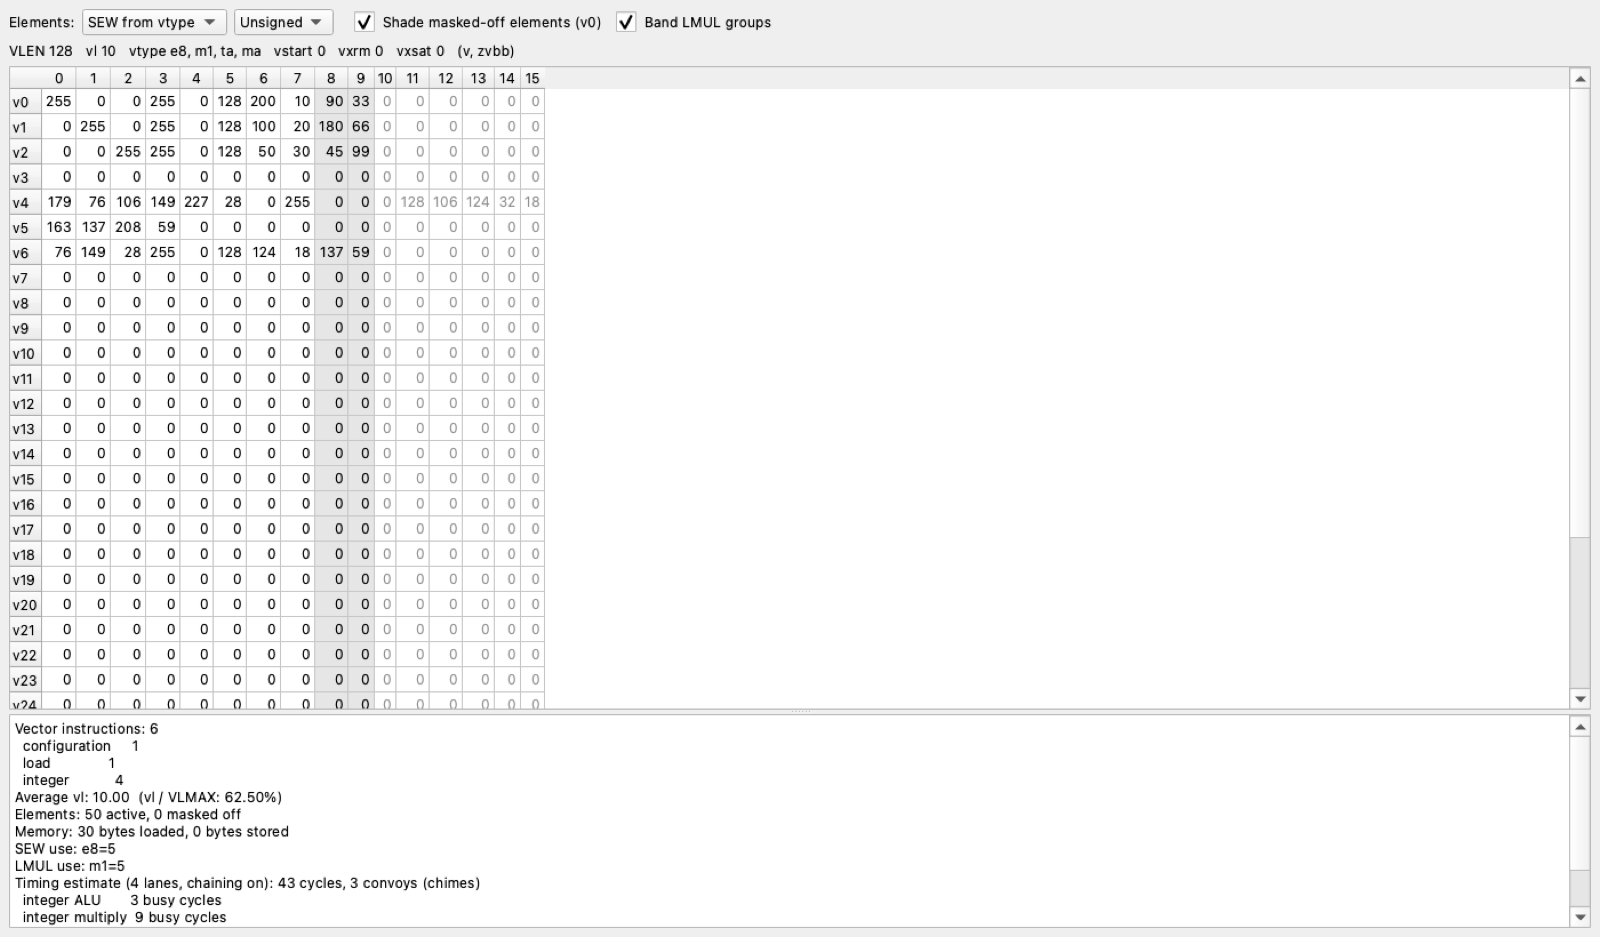
\includegraphics[width=\textwidth]{figures/vector_tab.png}
\caption{Vector tab in \texttt{rgb\_to\_grey.s} (unsigned, mask shading on). \insn{vlseg3e8.v} has
split the pixels into R, G and B in \texttt{v0}--\texttt{v2}; elements at or beyond
\texttt{vl}\,=\,10 are dimmed; elements 8 and 9 are shaded because their \texttt{v0} bits are 0;
the statistics and timing estimate are below.}\label{fig:tab}
\end{figure}

\begin{figure}[H]
\centering
\begin{minipage}[t]{0.30\textwidth}\centering
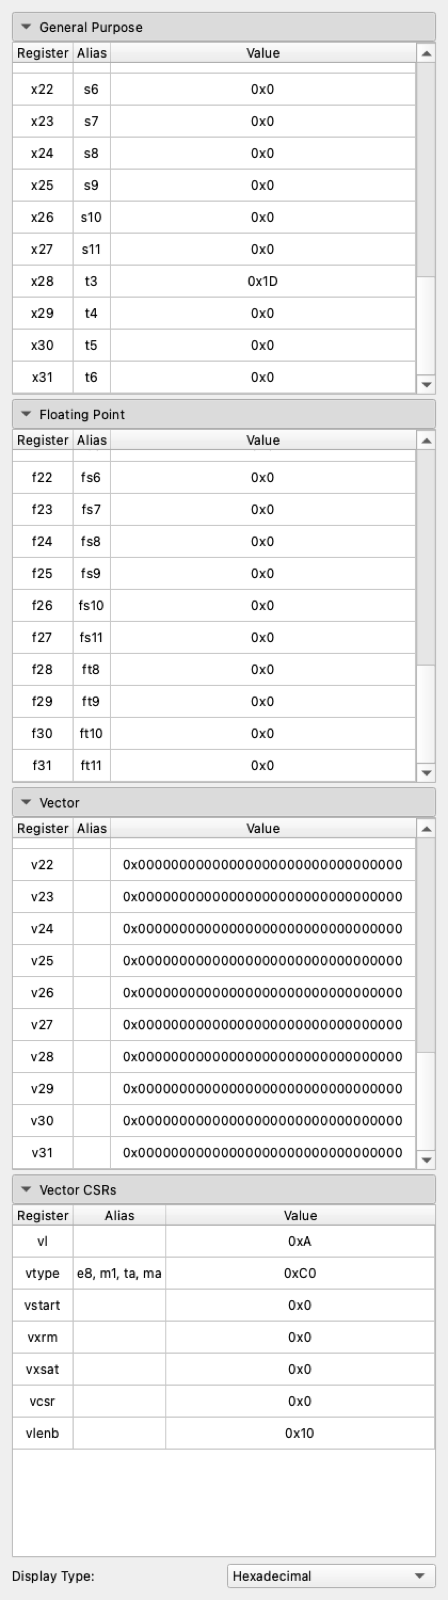
\includegraphics[width=\textwidth]{figures/register_panel.png}
\caption{Register panel, scrolled to the vector sections.}\label{fig:regs}
\end{minipage}\hfill
\begin{minipage}[t]{0.66\textwidth}\centering
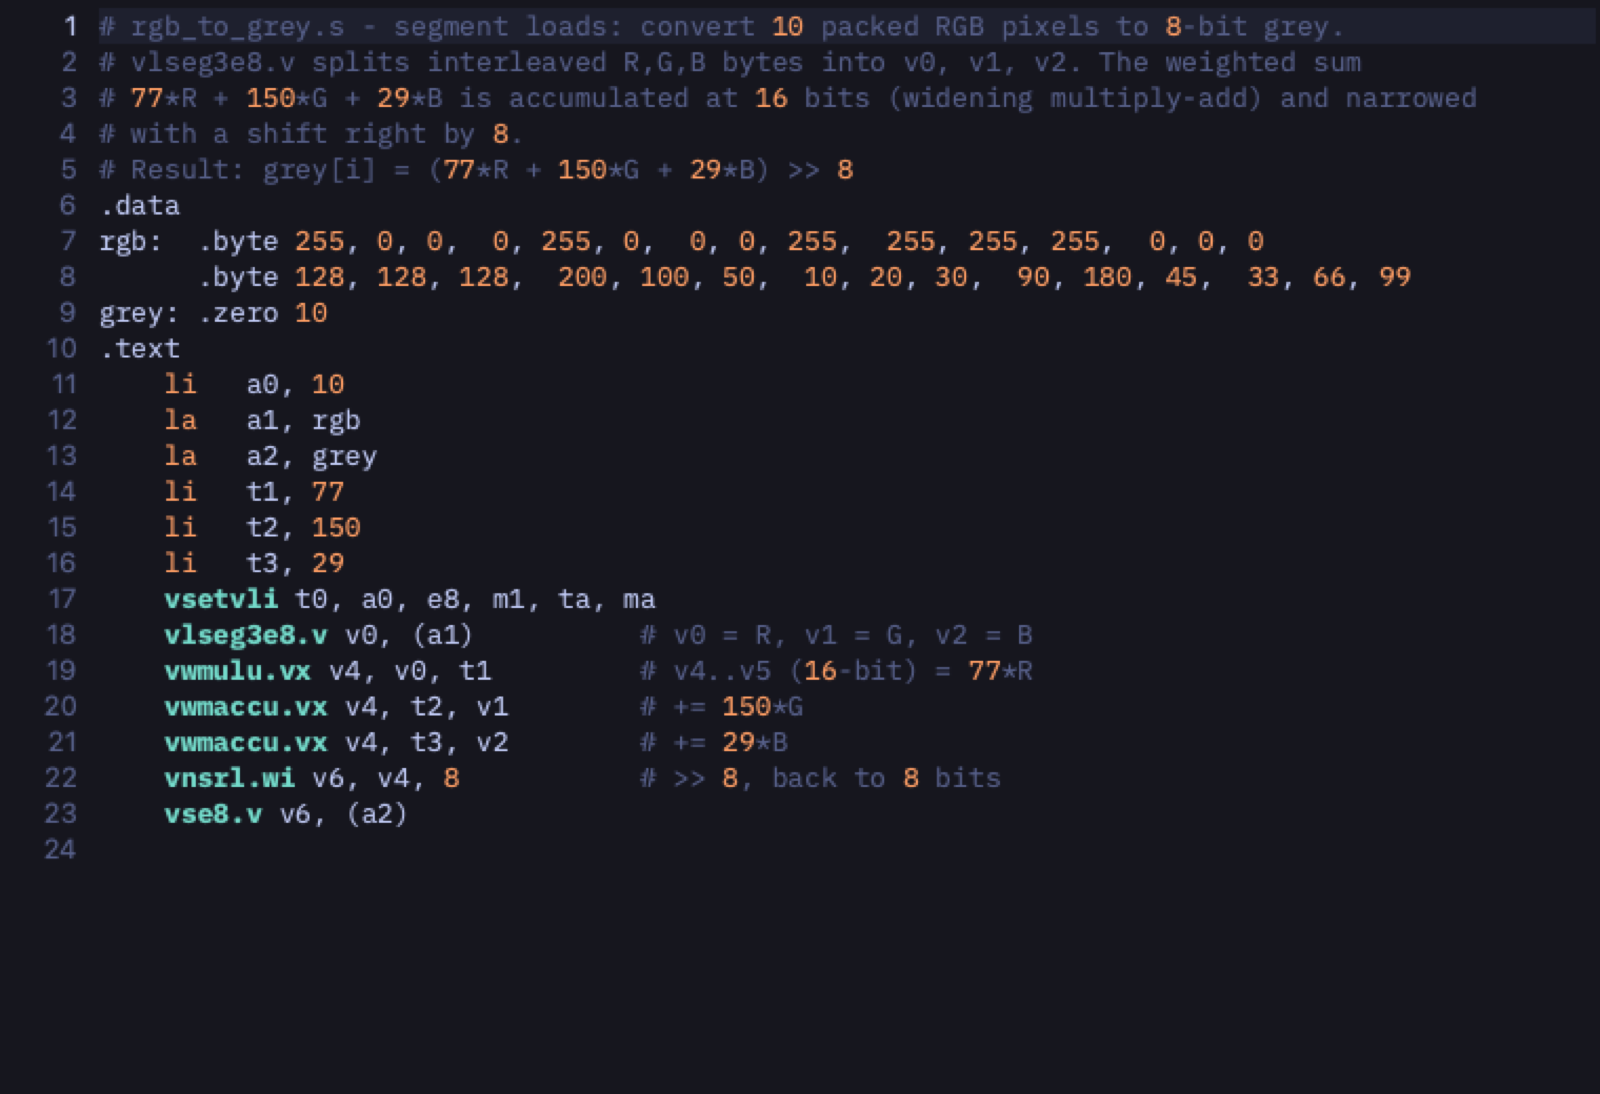
\includegraphics[width=\textwidth]{figures/editor_highlight.png}
\caption{Editor with vector code.}\label{fig:editor}
\end{minipage}
\end{figure}

\begin{figure}[H]
\centering
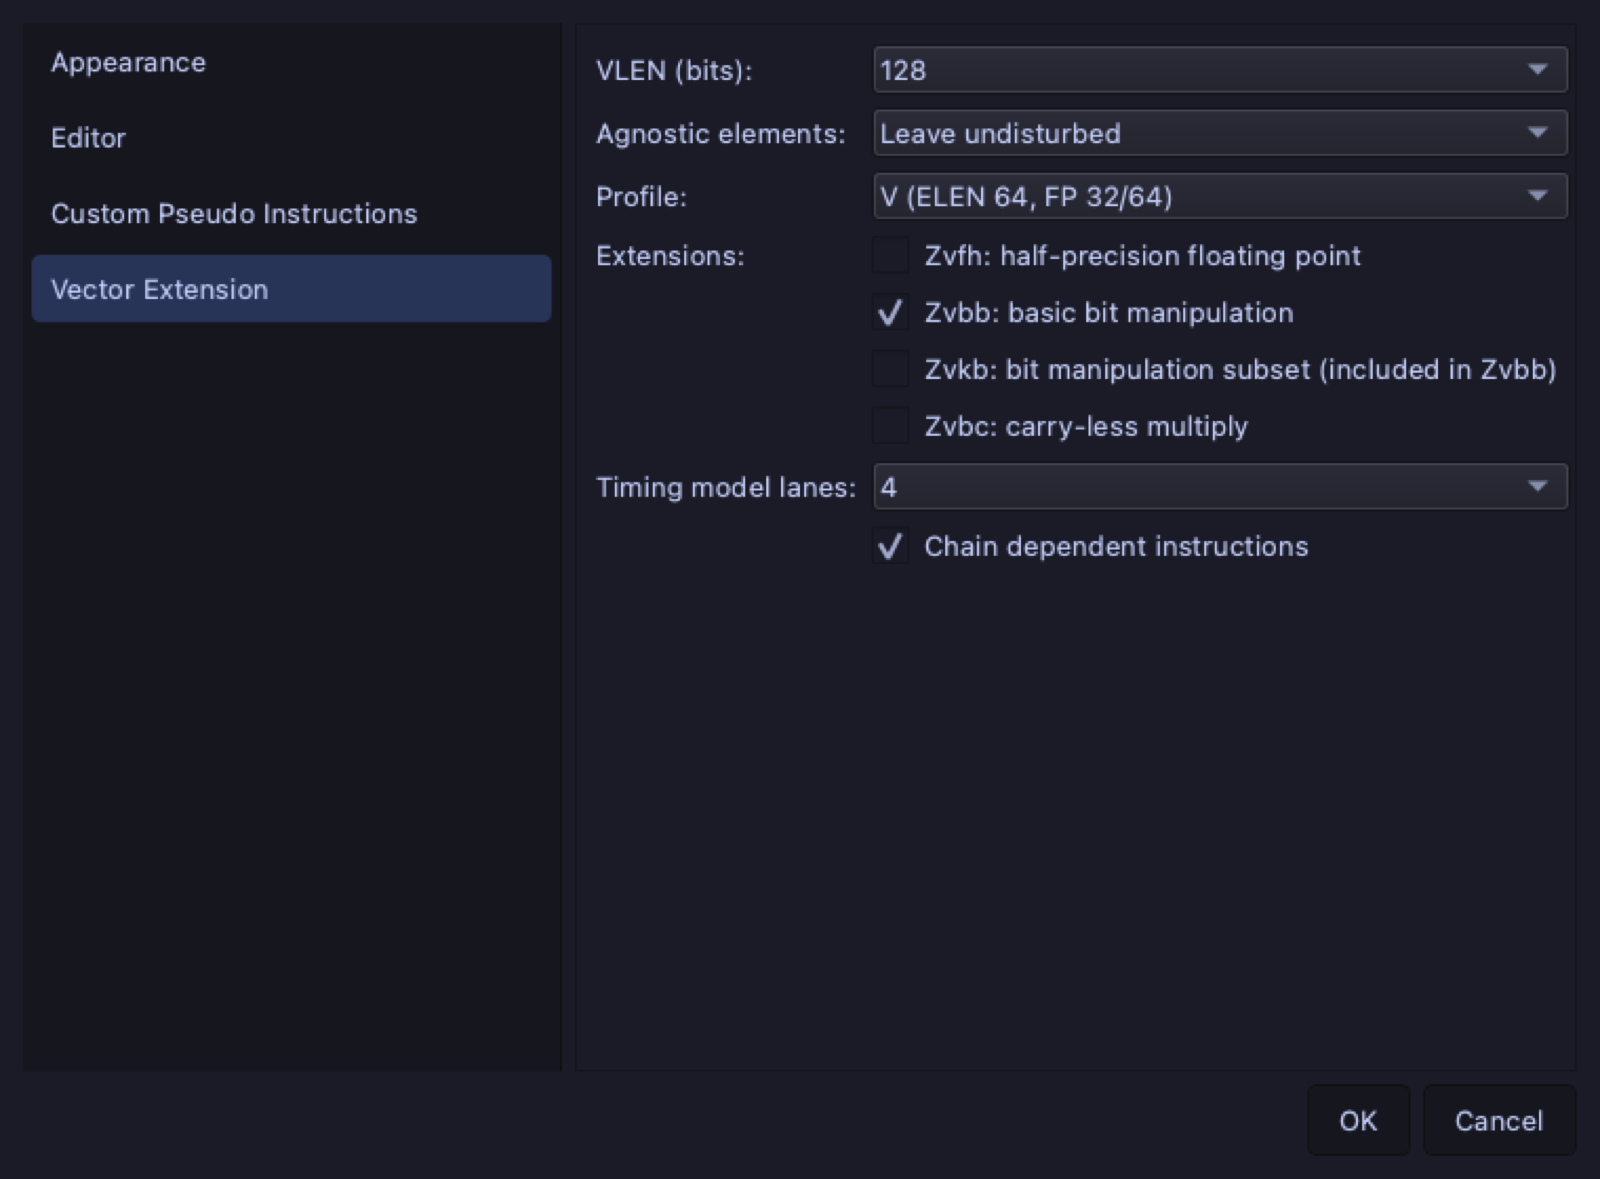
\includegraphics[width=0.62\textwidth]{figures/settings_vector.png}
\caption{Settings $\rightarrow$ Vector Extension.}\label{fig:settings}
\end{figure}

\begin{figure}[H]
\centering
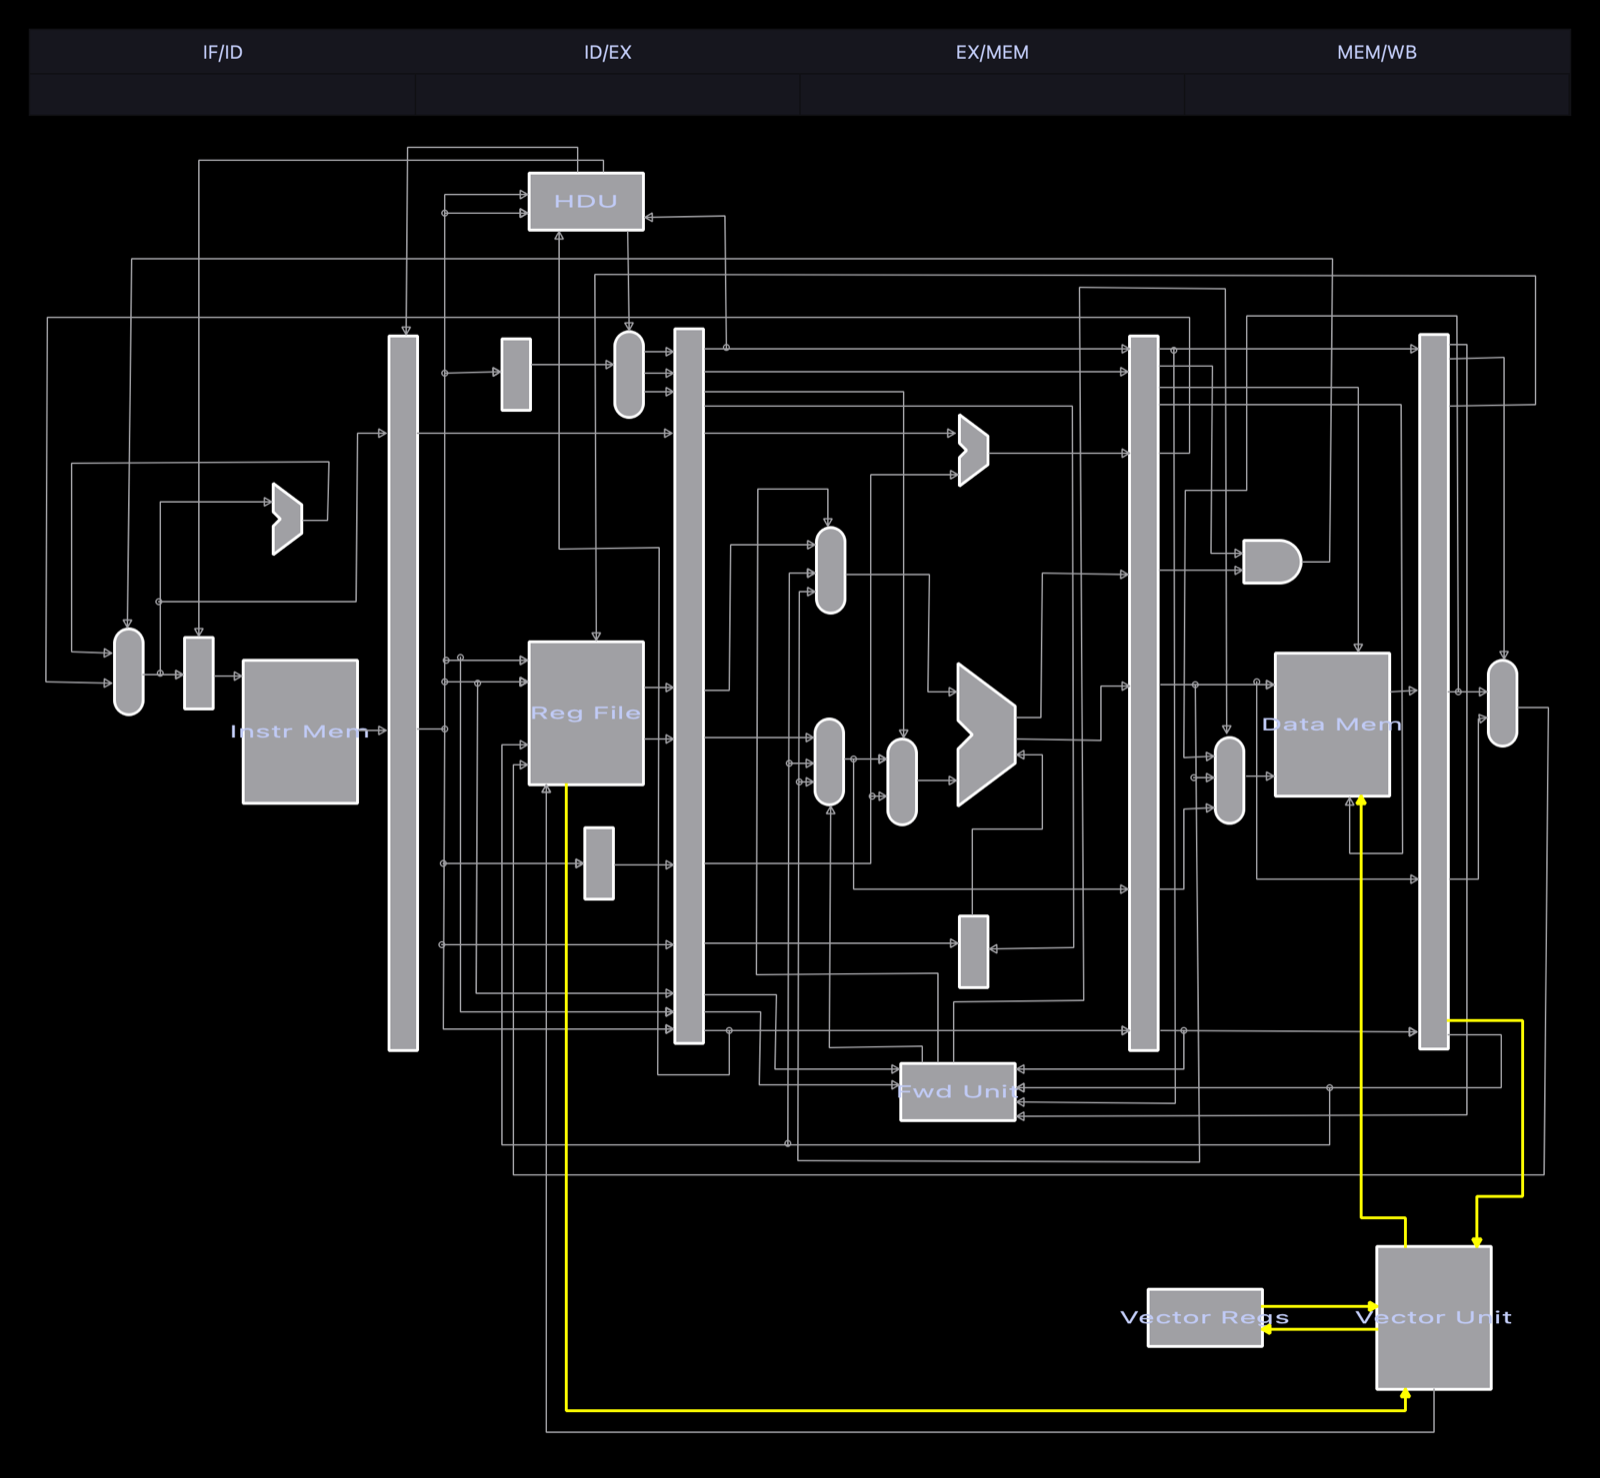
\includegraphics[width=0.85\textwidth]{figures/circuit_h_f.png}
\caption{Circuit view of the pipeline with hazard detection and forwarding; the vector unit and
its active wires (yellow) are at the bottom right.}\label{fig:circuit}
\end{figure}

% =====================================================================  8
\section{Defects}\label{sec:defects}

\subsection{In the existing Kites code}
Validation found the following defects in code that existed before this work. F16--F19 are
listed in the scope document; F20--F25 were found while validating the stretch goals.

\small
\begin{longtable}{@{}L{0.8cm}L{8.8cm}L{5.5cm}@{}}
\caption{Defects in the existing code.}\label{tab:defects}\\
\toprule
ID & Defect & Resolution \\
\midrule
\endfirsthead
\caption[]{Defects in the existing code (continued).}\\
\toprule
ID & Defect & Resolution \\
\midrule
\endhead
F16 & Scalar FP: $x/0$ gives NaN, flag bits reversed, NaN-to-integer not saturated, no RMM. & Reported; vector FP does not use these routines. \\
F17 & A label named \texttt{data}, \texttt{text} or \texttt{bss} hangs or breaks the assembler. & Reported; examples avoid the names. \\
F19 & \file{test/test_main.cpp} includes \texttt{windows.h} unconditionally. & Fixed. \\
F20 & Pipelines: AUIPC adds two register values, so \insn{la} gives wrong addresses; LUI is not sign-extended. & Fixed, regression tests. \\
F21 & Forwarding pipelines do not forward the integer source of F/D instructions (load/store base, \insn{fmv.w.x}, \insn{fcvt.s.w}). Found by the Spike campaign on H\_F (17 of 150 programs). & Fixed, regression test. \\
F22 & Pipelines pause at the end-of-program breakpoint while draining, so \texttt{kites-cli} never finishes on a pipeline model. & Fixed, regression test. \\
F23 & CSR instructions are no-ops on the pipelines (the execute stage returns early, which also repeats the previous instruction's MEM/WB on NH\_NF). & Fixed: CSRs execute in WB. \\
F24 & Custom pseudo-instructions: an operand list written as ``\texttt{a, b}'' is split into an empty operand, so the line is not expanded. & Fixed, tests. \\
F25 & The CMake \texttt{coverage} target links \texttt{libgcov}, which Apple Clang lacks. & Reported; source-based coverage used instead. \\
\bottomrule
\end{longtable}
\normalsize

\subsection{In the new code}
Defects in the vector code found during validation were fixed before the corresponding commit,
each with a test. The ones worth recording are: the unordered-sum NaN choice
(\cref{sec:spike-diff}); the pipeline stall needed for scalar FP instructions that follow a
vector or CSR instruction, so that \texttt{fflags} and \texttt{frm} are accessed in program order
(PL09); and the display of an illegal \texttt{vtype}, which the REPL and the viewer printed as a
raw number and now show as \texttt{vill}.

% =====================================================================  9
\section{Traceability}\label{sec:trace}

\small
\begin{longtable}{@{}L{1.9cm}L{7.0cm}L{4.4cm}L{1.2cm}@{}}
\caption{Requirements of the scope document and the stretch goals, with their tests.}\label{tab:trace}\\
\toprule
ID & Requirement (short) & Tests & Result \\
\midrule
\endfirsthead
\caption[]{Traceability (continued).}\\
\toprule
ID & Requirement (short) & Tests & Result \\
\midrule
\endhead
VS-01 & 32 vector registers of VLEN bits & VecConfig, VC03\_* & \pass \\
VS-02/03 & vector CSRs, read-only rules, \texttt{vcsr} & VS02\_VS03\_vector\_csrs & \pass \\
VS-04 & reset state & VS04\_reset\_state & \pass \\
VC-01/02/03 & \insn{vset*}, \texttt{x0} cases, \texttt{vill} & VC01\_*, VC02\_*, VC03\_* & \pass \\
VM-01/02 & unit-stride, strided, indexed & VM01\_*, VM01\_VM02\_* & \pass \\
VM-03 & mask and whole-register & VM03\_* & \pass \\
VM-04 & through the memory controller, undo & VM04\_*, SI02\_* & \pass \\
VM-05 & segment, fault-only-first & VM05\_*, examples & \pass \\
VA-01 & integer, reduction, mask, permutation & VA01\_* (16 tests) & \pass \\
VA-02 & division edge cases & VA02\_* & \pass \\
VA-03 & fixed point & VA01\_VA03\_*, fir\_q15 & \pass \\
VA-04 & floating point & VA04\_* & \pass \\
VA-05 & 7-bit estimates & VA05\_* & \pass \\
VP-01 & masking and policies & VA01\_*, VC04\_* & \pass \\
VP-02 & \texttt{vstart} & VP02\_*, VL02\_* & \pass \\
VL-01/02 & legality, state unchanged & VL01\_*, VL02\_*, PL07 & \pass \\
AS-01/02 & encodings, round trip & AS01\_*, AS02\_* & \pass \\
AS-03 & error messages & AS03\_* & \pass \\
AS-04 & labels named like vtype fields & AS04\_* & \pass \\
AS-05 & highlighting, completion & GUI checklist & \pass \\
AS-06 & pseudo-instructions & AS06\_* & \pass \\
SI-01 & retirement & SI01\_* & \pass \\
SI-02 & undo/redo & SI02\_*, PL08 & \pass \\
SI-03 & scalar F/D unaffected & existing FP suites, VecAsm & \pass \\
SI-04 & pipelines execute vector code (B1) & SI04\_*, PL01--PL09 & \pass \\
OB-01/02/03 & dump, register view, profiler type & examples, GUI checklist, VecAsm & \pass \\
NF-01 & scalar performance & \cref{sec:perf} & \pass \\
NF-02 & builds; portable 128-bit multiply & macOS build; helpers & \partly \\
NF-03 & conventions, comments & review & \pass \\
NF-04 & coverage & \cref{sec:coverage} & \pass \\
\midrule
B1 & pipelined execution & VecPipeline, Spike on H\_NF/H\_F & \pass \\
B2 & timing model & VT01\_* & \pass \\
B3 & vector viewer & GUI checklist & \pass \\
B4 & VLEN, agnostic fill & VC03\_*, VC04\_*, Spike at 4 VLENs & \pass \\
B5 & statistics & VS01\_* & \pass \\
B6 & random differential testing & \cref{sec:spike} & \pass \\
B7 & circuit view & GUI checklist & \pass \\
B8 & Zvfh, Zvbb/Zvkb, Zvbc, Zve* & VX01--VX04, VecHalf, Spike & \pass \\
B9 & CLI and REPL commands & manual run, Spike harness & \pass \\
B10 & custom vector pseudo-instructions & VectorCustomPseudo & \pass \\
\bottomrule
\end{longtable}
\normalsize

% =====================================================================  10
\section{Quality gates}\label{sec:gates}

\begin{table}[H]
\centering\small
\caption{Quality gates of the scope document.}\label{tab:gates}
\begin{tabularx}{\textwidth}{@{}L{1.0cm}YL{1.4cm}@{}}
\toprule
Gate & Evidence & Status \\
\midrule
QG1 & every table entry has a golden encoding (inventory test); every instruction family has semantic tests and appears in the random Spike programs & \pass \\
QG2 & 261/261 tests pass; every deviation is documented (design document, limitations) & \pass \\
QG3 & 95.2\,\% lines, 88.5\,\% branches & \pass \\
QG4 & all examples match Spike on three processors and four VLENs & \pass \\
QG5 & existing suite passes on macOS; Linux and Windows were not available & \partly \\
QG6 & undo/redo round trips for the examples on the single-cycle processor and a pipeline & \pass \\
QG7 & GUI checklist and renders (\cref{sec:gui}) & \pass \\
\bottomrule
\end{tabularx}
\end{table}

% =====================================================================  11
\section{Limitations}\label{sec:limits}

The known limitations are listed in the design document: RMM arithmetic for single and double
precision rounds ties to even, underflow for those widths follows the host's tininess rule,
scalar single and half values are not NaN-boxed, there are no traps, the pipeline models without
hazard detection need two instructions between a vector or CSR result and its scalar use, and
the timing model is an estimate. Validation used one platform (macOS on arm64).

% =====================================================================  12
\section{Reproducing the results}\label{sec:repro}

\begin{lstlisting}[language={},basicstyle=\ttfamily\scriptsize]
# tests
cmake -S . -B build/test -G Ninja -DENABLE_TESTS=ON -DDISABLE_GUI=ON -DCMAKE_PREFIX_PATH=$(brew --prefix qt)
cmake --build build/test && (cd build/test && ctest)

# differential testing (needs spike, llvm-mc, ld.lld)
python3 -I tools/vector/spike_diff.py --kites build/test/kites-cli examples examples/vector/*.s
python3 -I tools/vector/spike_diff.py --kites build/test/kites-cli random --count 500 --seed 1
python3 -I tools/vector/spike_diff.py --kites build/test/kites-cli --vm rv5-h-f --vlen 256 \
    --vector-ext v,zvfh,zvbb,zvbc random --count 100 --seed 17001

# coverage (Apple Clang)
cmake -S . -B build/cov -G Ninja -DENABLE_TESTS=ON -DDISABLE_GUI=ON -DCMAKE_PREFIX_PATH=$(brew --prefix qt) \
    -DCMAKE_CXX_FLAGS="-fprofile-instr-generate -fcoverage-mapping" \
    -DCMAKE_C_FLAGS="-fprofile-instr-generate -fcoverage-mapping" -DCMAKE_EXE_LINKER_FLAGS="-fprofile-instr-generate"
cmake --build build/cov --target kites_test
(cd build/cov && LLVM_PROFILE_FILE="$PWD/prof/%p.profraw" ctest)
xcrun llvm-profdata merge -sparse build/cov/prof/*.profraw -o build/cov/kites.profdata
xcrun llvm-cov report build/cov/test/kites_test -instr-profile=build/cov/kites.profdata \
    src/processor/vector src/assembler/parse_formats/v_formats.cpp
\end{lstlisting}

% =====================================================================  REFERENCES
\begin{thebibliography}{99}\small\markboth{References}{References}
\bibitem{spec} RISC-V International. \emph{The RISC-V Instruction Set Manual, Volume I: Unprivileged
  Architecture}, ``V'' Standard Extension for Vector Operations, version 1.0.
  \url{https://docs.riscv.org/reference/isa/v20260120/unpriv/v-st-ext.html}
\bibitem{spike} RISC-V Software. \emph{Spike RISC-V ISA Simulator}.
  \url{https://github.com/riscv-software-src/riscv-isa-sim}
\bibitem{llvm} LLVM Project. \emph{User Guide for RISC-V Target} and \texttt{llvm-mc}.
  \url{https://llvm.org/docs/RISCVUsage.html}
\end{thebibliography}

\end{document}
